%\input{tcilatex}
%\input{tcilatex}


\documentclass[a4paper,10pt]{article}
%%%%%%%%%%%%%%%%%%%%%%%%%%%%%%%%%%%%%%%%%%%%%%%%%%%%%%%%%%%%%%%%%%%%%%%%%%%%%%%%%%%%%%%%%%%%%%%%%%%%%%%%%%%%%%%%%%%%%%%%%%%%%%%%%%%%%%%%%%%%%%%%%%%%%%%%%%%%%%%%%%%%%%%%%%%%%%%%%%%%%%%%%%%%%%%%%%%%%%%%%%%%%%%%%%%%%%%%%%%%%%%%%%%%%%%%%%%%%%%%%%%%%%%%%%%%
\usepackage{amsfonts}
\usepackage[utf8]{inputenc}
\usepackage{indentfirst}
\usepackage{times}
\usepackage[T1]{fontenc}
\usepackage[affil-it]{authblk}
\usepackage{authblk}
\usepackage{amssymb,amsmath,amsthm,ragged2e}
\usepackage{setspace,lipsum}
\usepackage[pdftex]{color,graphicx}
\usepackage{adjustbox}
\usepackage{lmodern,caption}
\usepackage{booktabs,array}
\usepackage{epstopdf}
\usepackage{array,longtable}
\usepackage[top=3cm, bottom=2cm, left=3cm, right=2cm]{geometry}
\usepackage{latexsym,hhline}
\usepackage[round]{natbib}
\usepackage[colorlinks=true,allcolors=blue]{hyperref}
\usepackage{setspace}
\usepackage{tikz,color,listings,float,booktabs,enumerate,multirow,multicol,subcaption}
\usepackage{parskip}
\usepackage{bigstrut,hyperref,tabularx,ctable,array,longtable,tikz}
\usepackage{rotating}
\usepackage[listings]{tcolorbox}
\usepackage{fancyheadings,xspace,amsmath,tikz-qtree}
\usepackage[labelfont=bf]{caption}
\usepackage{threeparttable}
\usepackage{standalone}
\usepackage[pdftex]{color,graphicx}

\setcounter{MaxMatrixCols}{10}
%TCIDATA{OutputFilter=LATEX.DLL}
%TCIDATA{Version=5.50.0.2953}
%TCIDATA{<META NAME="SaveForMode" CONTENT="1">}
%TCIDATA{BibliographyScheme=BibTeX}
%TCIDATA{LastRevised=Saturday, March 18, 2017 04:40:50}
%TCIDATA{<META NAME="GraphicsSave" CONTENT="32">}

\DeclareGraphicsRule{.tif}{png}{.png}{`convert #1 `dirname #1`/`basename #1 .tif`.png}
\newcommand{\otoprule}{\midrule[\heavyrulewidth]}
\newcolumntype{Z}{>{\centering\arraybackslash}X}
\onehalfspacing
\DeclareMathOperator{\diag}{diag}
\DeclareMathOperator{\Ima}{Im}
\DeclareCaptionLabelSeparator{horse}{:\quad}
\captionsetup{
labelsep = horse,
figureposition = bottom }
\setlength{\parindent}{15pt}
\hypersetup{
pdftitle={TITLE},
pdfauthor={AUTHOR},
pdfsubject={SUBJECT},
pdfkeywords={KEYWORD} {KEYWORD} {KEYWORD},
colorlinks=true,
linkcolor=blue,
citecolor=blue,
filecolor=magenta,
urlcolor=blue
}
\newtheorem{theorem}{Theorem}
\newtheorem{proposition}{Proposition}
\newtheorem{lemma}{Lemma}
\newtheorem{definition}{Definition}
\newcommand{\R}{\mathbb R}
\newcommand{\Nat}{\mathbb N}
\newcommand{\C}{\mathbb C}
\newcommand{\Pstar}{\mathbb{P}^{\ast}}
\newcommand{\E}{\mathbb{E}}
\newcommand{\Var}{\mathrm{Var}}
\newcommand{\Cov}{\mathrm{Cov}}
\newcommand{\Expect}{{\rm I\kern-.3em E}}
\tcbuselibrary{listings,theorems}
\usetikzlibrary{matrix}
\newtheorem{corollary}{Corollary}[theorem]
%\input{tcilatex}

\begin{document}

\title{Worst Case CVaR Portfolio Optimization with Multidimensional Copulas}
\author[1]{Fernando A. Boeira Sabino da Silva\thanks{\texttt{Department of Statistics, Federal University of Rio Grande do Sul, Porto Alegre, RS 91509-900, Brazil, e-mail: fsabino@ufrgs.br
}; Corresponding author.} \and Flavio A. Ziegelmann\thanks{\texttt{%
Department of Statistics, Federal University of Rio Grande do Sul, Porto Alegre, RS 91509-900, Brazil, e-mail: flavioz@ufrgs.br}}\thanks{%
We thank Cristina Tessari for helpful discussions and for helping us
obtaining the data we use.}}
\date{}
\maketitle

\begin{abstract}
Using data from the S\&P 500 shares from 1990 to 2015, we measure the
downside market risk by Conditional Value-at-Risk (CVaR) subject to return
constraints following the approach of \citet*{rockafellar2000,rockafellar2002%
} and the extended framework of \citet*{kakouris14} through the use of
multidimensional mixed archimedean copulas. We implement a dynamic investing
strategy where the portfolios are optimized using three different length of
rolling calibration windows. The out-of-sample performance is evaluated and
compared against two benchmarks; a multidimensional gaussian copula model and a
constant mix portfolio. Our empirical analysis shows that the Mixed Copula-CVaR
approach generates portfolios with better downside risk statistics for any rebalancing period and it is more profitable than the Gaussian Copula-CVaR and 1/N portfolios for daily and weekly rebalancing. %Particularly, the mixture copula and benchmark
%methods show a mean annualized excess return as high as 11.29\%, 10.59\% and
%10.52\%. 
To cope with the dimensionality problem we employ a similar approach to that used by \citet*{ggr06} to select a set of assets that are the most
diversified, in some sense, to the S\&P 500 index in the constituent set. We find that copula-based approaches offer better hedges against losses than the 1/N portfolio. The accuracy of VaR forecasts is determined by how well they minimize a capital requirement loss function (CR). In order to mitigate data-snooping problems we apply a test for superior predictive ability (SPA) proposed by  \citet*{hansen2005test} to determine which model significantly minimizes this expected loss function. The test is implemented via stationary bootstrap of \citet*{pr94} using the automatic block-length selection of \citet*{pw04} and 10,000 bootstrap resamples. We find that the minimum average loss of the mixed Copula-CVaR approach is smaller than the average performance of the Gaussian Copula-CVaR.


\smallskip

\smallskip

\noindent \textbf{Keywords:} Asset Allocation; Capital Requirement Loss; Copula; Portfolio
Selection; Risk Management; S\&P 500; Superior Predictive Ability; Stationary Bootstrap; WCCVaR.

\noindent \textbf{JEL Codes:} C15; C52; C53; C61; C63; G11.
\end{abstract}

\makeatletter

\makeatother

\affil[1]{PPGE-UFRGS} \affil[2]{PPGE-UFRGS, PPGA-UFRGS}

%\date{July 25, 2016}

\section{Introduction}

\label{introduction}

The seminal article Portfolio Selection published by  \citet*{
	markowitz1952} introduces the foundation for modern portfolio theory (MPT) or mean-variance analysis. Markowitz considered the problem of an agent who wishes to find the maximum (expected) return for a given level of risk or minimize risk for a given level of return. He identified that, by diversifying a portfolio among investments
that have different return patterns, investors can build such an efficient
portfolio.

Quantile functions are commonly used for measuring the market risk of models
with parameter uncertainty and variability. Portfolio optimization involving
a mean-value-at-risk (mean-VaR) portfolio and the CVaR have been analyzed by %
\citet*{alexander2002} and \citet*{rockafellar2000}, respectively. Akin to
the classical Markowitz portfolio, in these approaches we want to determine
the weights that maximize the portfolio return for a specified VaR or CVaR
at a given confidence level or minimize these quantiles for a given
confidence level subject to a fixed portfolio return.

\citet*{artzner1999} show that VaR has undesirable properties such as lack
of sub-additivity and thus it is not a coherent measure. Furthermore, \citet*%
{uryasev2001} show that VaR may be a non-convex function with respect to
portfolio weights, which can yield to multiple portfolio local solutions,
but CVaR is coherent both for continuous and discrete distributions and it
is a convex function. In addition, they show that an outright optimization
with respect to CVaR is numerically difficult due to the dependence of the
CVaR on VaR. However, \citet*{rockafellar2000} show that VaR and CVaR can be
computed simultaneously, introducing auxiliary risk measures, and it can be
used in conjunction with scenario based optimization algorithms reducing the
problem to a linear programming problem which allows us to optimize a
portfolio with very large dimensions and stable numerical implementations.

A well-known problem of the Markowitz model is its sensitivity to the input parameters. In practice, the implementation of strategies based on the risk-return trade-off remains a fundamental challenge in many areas of financial management, since estimation errors of the expected returns of the assets and the covariance matrix of these returns can significantly affect cause an impact in the asset allocations weights, no longer leading to an efficient portfolio. This issue can be overcome by employing robust optimization and
worst case techniques \citet*{zhu2009worst} in which assumptions about the
distribution of the random variable are relaxed, and thus, we obtain the
optimal portfolio solution by optimizing over a prescribed feasible set and
possible densities. \citet*{kakouris14} show how copula-based models can be
introduced in the Worst Case CVaR (WCVaR) framework. This approach is
motivated by an investor's desire to be protected against the worst possible
scenario.

In this paper, we employ a similar methodology to that of \citet*{kakouris14}
and investigate the advantage of such dependence structure through an
empirical study. We evaluate the out-of-sample performance of the Worst Case Copula-CVaR and compare the relative performance of the strategy to the Gaussian Copula-CVaR, a naive 1/N (equally-weighted) and the S\&P 500
index in the long term in terms of wealth accumulation and downside risk.

The main novel contribution of this paper is to select a diversified set of assets that can be useful during crises and tranquil periods, i.e., that somehow involves hedging of decisions to protect the investors against any market conditions and evaluate the approaches using 50-dimensional archimedean and gaussian copula models without constructing hierarchical copulas.  

Our data set consists of daily data of adjusted closing prices of all
shares that belong to S\&P 500 market index from July 2st, 1990 to December
31st, 2015. We obtain the adjusted closing prices from Bloomberg. The data
set sample encompasses 6426 days and includes a total of 1100 stocks over
the whole period. We consider only stocks that are listed throughout a 48
plus 6-month period in the analysis, i.e., close to 500 stocks in each
trading period. Moreover, we consider alternative portfolio rebalancing
frequencies and return constraints. Returns are calculated in excess of a risk-free asset.

To be effective in
dealing with uncertainty, we select, among all listed assets in each
formation period, a set of 50 stocks based on the ranked sum of absolute
deviations (the twenty-five largest and smallest) between the normalized
daily closing prices deviations (known as distance) of the S\&P 500 index
and all shares, adjusting them by dividends, stock splits and other
corporate actions. By selecting a diversified set of assets that can be
useful during crises and tranquil periods we address the issue of asset
allocation taking into account the purpose of risk diversification. These
stocks are then evaluated over the next six months.

 Our backtest results indicate
that the Worst Case Copula-CVaR approach outperforms consistently the
benchmark strategies in the long term in terms of downside risk measured by VaR, CVaR and capital requirement loss. 

The remainder of the paper is structured as follows. In Section 2 we present
a general review, notations and definitions of the CVaR and mean-variance
optimization methodologies and extends them to our Worst Case framework
through the use of appropriate allowable and uncertainty sets. The data we
use is briefly discussed in Section 3. Section 4 summarizes the empirical
results of the analysis, while Section 5 concludes and provide further ideas
for research.

\section{Specifications of the Models under Analysis}

\label{section2}

\subsection{Conditional Value-at-Risk}

Let $Y$ be a stochastic vector standing for market uncertainties and $F_{Y}$
be its distribution function, i.e., $F_{Y}\left( u\right) =P\left( Y\leq
u\right) $. Let also $F_{Y}^{-1}\left( v\right) =\inf \left\{ u:F_{Y}\left(
u\right) \geq v\right\} $ be its right continuous inverse and assume that it
has a probability density function represented by $p(y)$\footnote{%
	This assumption can be relaxed \citep{uryasev2013}.}. Define the $VaR_{\beta
}$\thinspace\ as the $\beta $-quantile by
\begin{eqnarray}
VaR_{\beta }\left( Y\right) &=& \arg \min \left\{ \alpha \in
%TCIMACRO{\U{211d} }%
%BeginExpansion
\mathbb{R}
%EndExpansion
:P\left( Y\leq \alpha \right) \geq \beta \right\}  \label{one} \\
&=&F_{Y}^{-1}\left( \beta \right) \text{,}  \notag
\end{eqnarray}%
and the $CVaR_{\beta }$ as the solution to the following optimization
problem \citep{pflug2000}:
\begin{equation}
CVaR_{\beta }\left( Y\right) =\inf \left\{ \alpha \in
%TCIMACRO{\U{211d} }%
%BeginExpansion
\mathbb{R}
%EndExpansion
:\alpha +\frac{1}{1-\beta }E\left[ Y-\alpha \right] ^{+}\right\} \text{,}
\label{two}
\end{equation}%
where $\left[ t\right] ^{+}=\max \left( t,0\right) $.

\bigskip \citet*{uryasev1999} have shown that the $CVaR$ is the conditional
expectation of $Y$, given that $Y\geq VaR_{\beta }$, i.e.,
\begin{equation}
CVaR_{\beta }\left( Y\right) =\mathbb{E}\left( Y\left\vert Y\geq VaR_{\beta
}\left( Y\right) \right. \right) .  \label{three}
\end{equation}

Let $f\left( x,y\right) $ be a loss function \ depending upon a decision
vector $x$ that belongs to any arbitrarily chosen subset $X\in
%TCIMACRO{\U{211d} }%
%BeginExpansion
\mathbb{R}
%EndExpansion
^{n}$ and a random vector $y\in
%TCIMACRO{\U{211d} }%
%BeginExpansion
\mathbb{R}
%EndExpansion
^{m}$. In a portfolio optimization problem, the decision vector $x$ can be a
vector of portfolios' weights, $X$ be a set of feasible portfolios,
subject to linear constraints\footnote{%
	For example, we can assume a portfolio $X$ that does not allow short-selling positions (all $x_{i}\geq 0$, for $i=1,...,n$),
	that be fully invested, i.e., the total portfolio weights sum
	up to unity and that the expected return be greater than an arbitrary value $%
	R$.} and $y$ a vector that stands for market variables that can affect the loss.

\bigskip

For each $x$, the loss function $f\left( x,y\right) $ is a random variable
defined on a probability space $\left( \Omega ,\mathcal{F},P_{\mathcal{F}%
}\right) $ having a probability distribution on $\left(
%TCIMACRO{\U{211d} }%
%BeginExpansion
\mathbb{R}
%EndExpansion
,\mathcal{B},P_{\mathcal{B}}\right) $ induced by that of $y$, where $\left(
%TCIMACRO{\U{211d} }%
%BeginExpansion
\mathbb{R}
%EndExpansion
,\mathcal{B},P_{\mathcal{B}}\right) $ stands for a Borel probability space
including, therefore, the open and closed intervals in $%
%TCIMACRO{\U{211d} }%
%BeginExpansion
\mathbb{R}
%EndExpansion
$. The underlying distribution of $y\in
%TCIMACRO{\U{211d} }%
%BeginExpansion
\mathbb{R}
%EndExpansion
^{m}$ is assumed to have a density $p(y)$ and let the probability of $f\left( x,y\right) $ not exceeding some threshold $\alpha$ be denoted by
\begin{equation}
F(x,\alpha)=\int_{f(x,y)\leq \alpha}p(y)\,dy,  \label{four}
\end{equation}
where $F(x,\alpha)$ is the cumulative distribution function for the loss function $f\left( x,y\right) $, non-decreasing and right-continuous with respect to $\alpha$.

Using the previously defined notation $\left( \ref{two}\right) $ we can
write the $CVaR$ function, at confidence level $\beta $, by%
\begin{equation}
CVaR_{\beta }\left( x\right) = \frac{1}{1-\beta }\int_{f(x,y)\geq VaR_{\beta
	}\left( x\right) }f(x,y)p(y)dy\text{,}  \label{five}
\end{equation}

The optimization of $CVaR$ is difficult because of the presence of the $VaR$
in its definition (it requires the use of the nonlinear function max) in
this infinite dimensional problem. The main contribution of \citet*{%
	rockafellar2000} was to define a simpler auxiliary function
\begin{equation}
F_{\beta }\left( x,\alpha \right) = \alpha +\frac{1}{1-\beta }%
\int_{f(x,y)\geq \alpha }\left( f(x,y)-\alpha \right) p(y)dy\text{,}
\label{six}
\end{equation}%
which can be used instead of $CVaR$ directly, without need to compute $VaR$
first due to the following proposition (\citet*{pflug2000}): \bigskip

\begin{proposition}
	The function $F_{\beta }\left( x,\alpha \right) $ is convex with respect to $%
	\alpha $. In addition, minimizing $F_{\beta }\left( x,\alpha \right) $ with
	respect to $\alpha $ gives $CVaR$ and $VaR$ is a minimum point of this
	function with respect to $\alpha $, i.e.
	\begin{equation}
	\underset{\alpha \in
		%TCIMACRO{\U{211d} }%
		%BeginExpansion
		\mathbb{R}
		%EndExpansion
	}{\min }~F_{\beta }\left( x,\alpha \right) =F_{\beta }\left( x,VaR_{\beta
	}\left( x\right) \right) =CVaR_{\beta }(x)  \label{seven}
	\end{equation}
\end{proposition}

Moreover, we can use $F_{\beta }\left( x,\alpha \right) $ to find the optimal weights, $CVaR$ and
$VaR$ simultaneously over an allowable feasible set, i.e.,
\begin{equation}
\underset{x\in X}{\min }~CVaR_{\beta }(x)=\underset{}{\underset{\left(
		x,\alpha \right) \in X\times
		%TCIMACRO{\U{211d} }%
		%BeginExpansion
		\mathbb{R}
		%EndExpansion
	}{\min }F_{\beta }\left( x,\alpha \right) }.  \label{eight}
\end{equation}

\citet*{pflug2000} show that under quite general conditions $F_{\beta
}\left( x,\alpha \right) $ is a smooth function. In addition, if $f(x,y)$ is
convex with respect to $x$, then $F_{\beta }\left( x,\alpha \right) $ is
also convex with respect to $x$. Hence, if the allowable set $X$ is also
convex, we then have to solve a smooth convex optimization problem.

\subsection{Optimization Problem}

Assume that the analytical representation for the density $p(y)$ is not
available, but we can approximate $F_{\beta }\left( x,\alpha \right) $ using
$J$ scenarios, $y_{j}$, $j=1,...,J$ which are sampled from the density
function $p(y)$. Then, we approximate
\begin{eqnarray}
F_{\beta }\left( x,\alpha \right) &=&\alpha +\frac{1}{1-\beta }%
\int_{f(x,y)\geq \alpha }\left( f(x,y)-\alpha \right) p(y)dy  \notag \\
&=&\alpha +\frac{1}{1-\beta }\int_{y\in
	%TCIMACRO{\U{211d} }%
	%BeginExpansion
	\mathbb{R}
	%EndExpansion
	^{m}}\left( f(x,y)-\alpha \right) ^{+}p(y)dy  \label{fb}
\end{eqnarray}%
by its discretized version
\begin{equation*}
\widetilde{F}_{\beta }\left( x,\alpha \right) =\alpha +\frac{1}{\left(
	1-\beta \right) J}\sum_{j=1}^{J}\left( f(x,y_{j})-\alpha \right) ^{+}.
\end{equation*}%
Assuming that the feasible set $X$ and the loss
function $f(x,y_{j})$ are convex and the same for the loss
function $f(x,y_{j})$, we solve the following convex optimization problem:
\begin{equation}
\underset{x\in X,\alpha \in
	%TCIMACRO{\U{211d} }%
	%BeginExpansion
	\mathbb{R}
	%EndExpansion
}{\min }\widetilde{F}_{\beta }\left( x,\alpha \right) .  \label{ten}
\end{equation}

In addition, if the loss function $f(x,y)$ is linear with respect to
\thinspace $x$, then the optimization problem $\left( \ref{ten}\right) $
reduces to the following linear programming (LP) problem:%

%\begin{equation} 
\begin{alignat}{4}
& \underset{x \in \mathbb{R}^{n},z\in 	\mathbb{R}^{J},\alpha \in \mathbb{R}}{\text{minimize}}
& & \alpha +\frac{1}{\left( 1-\beta \right)  J}\sum_{j=1}^{J}z_{j}
\\ 
& \text{subject to} 
& & x\in X,\\
&&& z_{j}\geq f(x,y_{j})-\alpha , \\
&&& z_{j}\geq 0, \; j = 1, \ldots, J.
\end{alignat}
%\end{equation}
%\begin{align}
%\underset{x\in
%	%TCIMACRO{\U{211d} }%
%	%BeginExpansion
%	\mathbb{R}
%	%EndExpansion
%	^{n},z\in
%	%TCIMACRO{\U{211d} }%
%	%BeginExpansion
%	\mathbb{R}^{J},\alpha \in \mathbb{R}
%	%EndExpansion
%}{\min }\alpha +\frac{1}{\left( 1-\beta \right) J}\sum_{j=1}^{J}z_{j}\\
%%\label{eleven}
%\text{subject to }x\in X,\\\label{12}
%z_{j}\geq f(x,y_{j})-\alpha ,\\z_{j}\geq 0,\text{ }j=1,...,J,
%\label{13}
%\end{align}
where $z_{j}$ are indicator variables. By solving the LP problem above we
find the optimal decision vector, $x^{\ast }$, the optimal $VaR$, $\alpha
^{\ast }$, and consequently the optimal $CVaR$, $\widetilde{F}_{\beta
}\left( x=x^{\ast },\alpha=\alpha ^{\ast }\right) $.

Therefore, the optimization problem can be solved using algorithms that are
capable of solving efficiently very large-scale problems with any
distribution within reasonable time and high reliability as, for example,
simplex or interior point methods.

In the next subsections we assume that there are $n$ risky assets and denote
by $r$ their random (log)returns vector, i.e., $\mathbf{r}\mathbf{=}\left(
r_{1},...,r_{n}\right) ^{\top }$, with expected returns $\mathbf{\mu }%
\mathbf{=}\left( \mu _{1},...,\mu _{n}\right) ^{\top }$ and covariance
matrix $\Sigma _{nxn}$. Let also $r_{f}$ represent the risk-free asset
returns and the decision (portfolio's weights) vector by $\mathbf{w}\mathbf{=%
}\left( w_{1},...,w_{n}\right) ^{\top }$. Also assume that $\mathbf{w}\in
\mathcal{W}$, where $\mathcal{W}$ is a feasible set and that the portfolio
return loss function $f_{L}\left( \mathbf{w,r}\right) $ is a convex (linear)
function given by

\begin{equation*}
f_{L}(\mathbf{w},\mathbf{r})=\mathbf{w}^{^{\top }}\mathbf{r}\text{.}
\end{equation*}

By definition, the portfolio return is the negative of the loss, i.e., $-%
\mathbf{w}^{^{\top }}\mathbf{r}$.

\subsection{Worst Case CVaR}

Assume now that we do not have precise information about the distribution of
the random vector $\mathbf{r}$, but that its density belongs to a family of
distributions $\mathcal{P}$ defined by
\begin{equation}
\mathcal{P=}\left\{ \mathbf{r}\left\vert \mathbb{E(}\mathbf{r})=\mathbf{\mu }
,Cov(\mathbf{r})=\Sigma \right. \right\} ,  \label{13b}
\end{equation}
where $\Sigma$ is a positive definite matrix.

Instead of assuming the precise distribution of the random vector $r$,
\citet
*{zhu2009worst} consider the case where the probability distribution $\pi$
is only known to belong to a certain set, say $\mathcal{P}$, defined the
worst-case CVaR (WCVaR) as the CVaR when the worst-case probability
distribution in the set $\mathcal{P}$ occurs.

\bigskip

\begin{definition}
	Given a confidence level $\beta ,$ $\beta \in (0,1),$ the worst-case CVaR
	for fixed $w\in \mathcal{W}$ with respect to the uncertainty set $\mathcal{P}
	$ is defined as
	\begin{eqnarray}
	WCVaR_{\beta }\left( \mathbf{w}\right) &\equiv &\underset{\pi \in \mathcal{P}%
	}{\sup }~ CVaR_{\beta }\left( \mathbf{w}\right)  \notag \\
	&=&\underset{\pi \in \mathcal{P}}{\sup }~\underset{\alpha \in
		%TCIMACRO{\U{211d} }%
		%BeginExpansion
		\mathbb{R}
		%EndExpansion
	}{\min }~F_{\beta }\left(\mathbf{w},\alpha \right)  \label{14}
	\end{eqnarray}
\end{definition}

\citet*{zhu2009worst} further investigated the WCVaR risk measure with
several structures of uncertainty in the underlying distribution. In
particular, \citet*{zhu2009worst} consider the case where the distribution
of $r$ belong to a set of distributions consisting of all mixtures of some
possible distribution scenarios, i.e.,
\begin{equation}
p\left( \cdot \right) \in \mathcal{P}_{M}\equiv \left\{ \sum_{i=1}^{d}\pi
_{i}p^{i}\left( \cdot \right) :\sum_{i=1}^{d}\pi _{i}=1,\text{ }\pi _{i}\geq
0,\text{ }i=1,...,d\right\} ,  \label{15}
\end{equation}%
where $p^{i}\left( \cdot \right) $ denotes the $j$-th likelihood
distribution and define
\begin{eqnarray}
G_{\beta }\left( \mathbf{w},\alpha ,\pi \right) &=&\alpha +\frac{1}{1-\beta }%
\int_{\mathbf{r}\in
	%TCIMACRO{\U{211d} }%
	%BeginExpansion
	\mathbb{R}
	%EndExpansion
	^{n}}\left( f(\mathbf{w},\mathbf{r})-\alpha \right) ^{+}\sum_{i=1}^{d}\pi
_{i}p^{i}(\mathbf{r})d\mathbf{r},\text{ }j=1,...,J  \notag \\
&=&\sum_{i=1}^{d}\pi _{i}G_{\beta }^{i}\left( \mathbf{w},\alpha \right) ,%
\text{ }i=1,...,d,  \label{16}
\end{eqnarray}%
where%
\begin{equation}
G_{\beta }^{i}\left( \mathbf{w},\alpha \right) =\alpha +\frac{1}{1-\beta }%
\int_{\mathbf{r}\in
	%TCIMACRO{\U{211d} }%
	%BeginExpansion
	\mathbb{R}
	%EndExpansion
	^{n}}\left( f(\mathbf{w},\mathbf{r})-\alpha \right) ^{+}p^{i}(\mathbf{r})d%
\mathbf{r},\text{ }i=1,...,d.  \label{17}
\end{equation}%

\vspace{0.3cm}
By theorem 1 of \citet*{zhu2009worst} we can state that for each fixed $%
\mathbf{w}\in \mathcal{W}$,
\begin{eqnarray}
WCVaR_{\beta }\left( \mathbf{w}\right) &=&\underset{}{\underset{\alpha \in
		%TCIMACRO{\U{211d} }%
		%BeginExpansion
		\mathbb{R}
		%EndExpansion
	}{\min }~\underset{\pi \in \Pi }{\max }}~G_{\beta }\left( \mathbf{w},\alpha
,\pi \right)  \notag \\
&=&\underset{}{\underset{\alpha \in
		%TCIMACRO{\U{211d} }%
		%BeginExpansion
		\mathbb{R}
		%EndExpansion
	}{\min }~\underset{\pi \in \Pi }{\max }}\sum_{i=1}^{d}\pi _{j}G_{\beta
}^{i}\left( \mathbf{w},\alpha \right) .  \label{18}
\end{eqnarray}%
Thus, minimizing the worst-case CVaR over $w\in \mathcal{W}$ is equivalent
to the following min-min-sup optimization problem:
\begin{equation}
\underset{}{\underset{\mathbf{w}\in \mathcal{W}}{\min }}~WCVaR_{\beta
}\left( \mathbf{w}\right) =\underset{}{\underset{\mathbf{w}\in \mathcal{W}}{%
		\min }~\underset{\alpha \in
		%TCIMACRO{\U{211d} }%
		%BeginExpansion
		\mathbb{R}
		%EndExpansion
	}{\min }~\underset{\pi \in \Pi }{\sup }}~G_{\beta }\left( \mathbf{w},\alpha
,\pi \right) .  \label{19}
\end{equation}%
\citet*{zhu2009worst} also proved that WCVaR is a coherent risk measure and
it clearly satisfies $WCVaR_{\beta }\left( \mathbf{w}\right) \geq
CVaR_{\beta }\left( \mathbf{w}\right) \geq VaR_{\beta }\left( \mathbf{w}%
\right) $. Thus, $WCVaR_{\beta }\left( \mathbf{w}\right) $ can be
effectively used as a risk measure.

\bigskip

In the next subsections we provide a brief review of copulas and consider
the augmented framework of \citet*{kakouris14} to compute WCVaR through the
use of multidimensional mixture archimedean copulas.

\subsection{Copulas}

Copulas are often defined as multivariate distribution functions whose
marginals are uniformly distributed on $[0,1]$. In other words, a copula $C$
is a function such that
\begin{equation}
C\left( u_{1},...,u_{n}\right) =P\left( U_{1}\leq u_{1},...,U_{n}\leq
u_{n}\right) ,  \label{20}
\end{equation}%
where $U_{i}\sim U[0,1]$ and $u_{i}$ are realizations of $U_{i}$, $i=1,...,n$%
. The margins $u_{i}$ can be replaced by $F_{i}\left( x_{i}\right) $, where $%
x_{i}$, $i=1,...,n$ is a realization of a (continuous) random variable,
since they both belong to the domain $[0,1]$ and are uniformly distributed
by its probability integral transform (note that $P\left( F\left( x\right)
\leq u\right) =P\left( x\leq F^{-1}\left( u\right) \right) =F\left(
F^{-1}\left( u\right) \right) =u$). Therefore, copulas can be used to model
the dependence structure and margins separately, and therefore provide more
flexibility.

\bigskip

Formally, we can define a copula function $C$ as follows. \bigskip

\begin{definition}
	An n-dimensional copula (or simply n-copula) is a function C with domain $%
	[0,1]^{n}$, such that:
\end{definition}

1. C is grounded an $n$-increasing;

2. C has marginal distributions $C_{k},$ $k=1,...,n,$ where $C_{k}(\mathbf{u}%
)=u$ for every $\mathbf{u}=\left( u_{1},...,u_{n}\right) $ in $[0,1]^{n}.$

\bigskip

Equivalently, an $n$-copula is a function
\begin{equation*}
C:[0,1]^{n}\rightarrow \lbrack 0,1]
\end{equation*}%
with the following properties:

(i) (grounded) For all $\mathbf{u}$ in $[0,1]^{n},$ $C(\mathbf{u})=0$, if at
least one coordinate of $\mathbf{u}$ is $0$ and $C(\mathbf{u})=u_{k}$, if
all the coordinates of $\mathbf{u}$ are $1$ except $u_{k};$

(ii) ($n$-increasing) For all $\mathbf{a}$ and $\mathbf{b}$ in $[0,1]^{n}$
such that $a_{i}\leq b_{i}$, for every $i,$ $V_{C}\left( \left[ a,b\right]
\right) \geq 0,$ where $V_{c}$ is called $C-$volume.

One of the main results of the theory of copulas is Sklar's Theorem \citet*{%
	sklar1959}.

\bigskip

\begin{theorem}
	(Sklar's Theorem) Let $X_{1},...,X_{n}$ be random variables with
	distribution functions $F_{1},...,F_{n}$, respectively. Then, there exists
	an n-copula C such that,
	\begin{equation}
	F\left( x_{1},...,x_{n}\right) =C\left( F_{1}\left( x_{1}\right)
	,...,F_{n}\left( x_{n}\right) \right) ,  \label{21} 
	\end{equation}
\end{theorem} 
\noindent for all $\mathbf{x}=\left( x_{1},...,x_{n}\right) \in
%TCIMACRO{\U{211d} }%
%BeginExpansion
\mathbb{R}
%EndExpansion
^{n}$. If $F_{1},...,F_{n}$ are all continuous, then the function $C$ is
unique; otherwise $C$ is determined only on $\Ima F_{1}\times ...\times \Ima %
F_{n}$. Conversely, if $C$ is an $n$-copula and $F_{1},...,F_{n}$ are
distribution functions, then the function $F$ defined above is an $n-$%
dimensional distribution function with marginals $F_{1},...,F_{n}$.

\bigskip

\begin{corollary}
	Let $F$ be an n-dimensional distribution function with continuous marginals $%
	F_{1},...,F_{n}$, and copula $C$. Therefore, for any $\mathbf{u}=\left(
	u_{1},...,u_{n}\right) $ in $\left[ 0,1\right] ^{n}$,
	\begin{equation}
	C\left( u_{1},...,u_{n}\right) =F\left( F_{1}^{-1}\left( u_{1}\right)
	,...,F_{n}^{-1}\left( u_{n}\right) \right) ,  \label{22}
	\end{equation}
	where $F_{i}^{-1}$, $i=1,...,n$ are the quasi-inverses of the marginals.
\end{corollary}

Using the Sklar's theorem and its corollary we can derive an important
relation between the probability density functions and copulas. Let $f$ be a
joint density function (of the $n-$dimensional distribution function $F$)
and $f_{1},...,f_{n}$ univariate density functions of the margins $%
F_{1},...,F_{n}$. Assuming that $F\left( \cdot \right) $ and $C\left( \cdot
\right) $ are differentiable, by $\left( \ref{21}\right) $ and $\left( \ref%
{22}\right) $
\begin{eqnarray}
\frac{\partial ^{n}F\left( x_{1},...,x_{n}\right) }{\partial
	x_{1}...\partial x_{n}} &\equiv &f\left( x_{1},...,x_{n}\right) =\frac{
	\partial ^{n}C\left( F_{1}\left( x_{1}\right) ,...,F_{n}\left( x_{n}\right)
	\right) }{\partial x_{1}...\partial x_{n}} \\
&=&c\left( u_{1},...,u_{n}\right) \prod_{i=1}^{n}f_{i}\left( x_{i}\right) .
\label{23}
\end{eqnarray}%
From a modelling perspective, Sklar's Theorem allow us to separate the
modeling of the marginals $F_{i}\left( x_{i}\right) $ from the dependence
structure, represented in $C$. The copula probability density function
\begin{equation}
c\left( u_{1},...,u_{n}\right) =\frac{f\left( x_{1},...,x_{n}\right) }{
	\prod_{i=1}^{n}f_{i}\left( x_{i}\right) }  \label{24}
\end{equation}%
is the ratio of the joint probability function to what it would have been
under independence. Thus, we can interpret the copula as the adjustment that
we need to make to convert the independence probability density function
into the multivariate density function. In other words, copulas decompose
the joint probability density function from its margins. Now we can estimate
the multivariate distribution in two parts: (i) finding the marginal
distributions; (ii) finding the dependency between the filtered data from
(i). 

Thereafter, copulas accommodate various forms of dependence through suitable choice of the copula ``correlation matrix'' since they conveniently separate marginals from dependence component. The methodology allows one to derive joint distributions from marginals, even when these are not normally distributed. In fact, copulas allow the marginal distributions to be modeled independently from each other, and no assumption on the joint behavior of the marginals is required, which provides a great deal of flexibility in modeling joint distributions.

\bigskip

The reader interested on the history of copulas is referred to \citet*{%
	schweizer2011} and \citet*{nelsen06}. For an extensive list of parametric
copula families see \citet*{joe97} and \citet*{nelsen06} and references
therein. After late 1990's the theory and application of copulas grew
enormously. \citet*{cherubini04} accounts for developments in finance and
stochastic processes.

Here we focus in a special class of copulas called Archimedean. An
Archimedean copula has the form
\begin{equation}
C\left( u_{1},...,u_{n}\right) =\psi \left( \psi ^{-1}\left( u_{1}\right)
+\psi ^{-1}\left( u_{2}\right) +...+\psi ^{-1}\left( u_{n}\right) \right) ,
\end{equation}%
for an appropriate generator $\psi \left( \cdot \right) $, where $\psi :%
\left[ 0,\infty \right] \rightarrow \left[ 0,1\right] $ and satisfies (i) $%
\psi (0)=1$ and $\psi (\infty )=0$; (ii) $\psi $ is $d$-monotone, i.e., $%
(-1)^{k}$d$^{k}\psi \left( s\right) $d$s^{k}\geq 0$ for $k\in \left\{
0,...,d-2\right\} $ and $(-1)^{d-2}$d$^{d-2}\psi \left( s\right) $d$s^{d-2}$
is decreasing and convex. Most of the copulas in this class has a closed
form. Moreover, each member has a single parameter that controls the degree
of dependence, which allow modeling dependence in arbitrarily high
dimensions with only one parameter.

The concept of tail dependence can be especially useful when dealing with
co-movements of assets. Studies on financial markets show that financial
assets have asymmetric distributions and heavy tails. Often elliptical
copulas, like gaussian and t-student copulas are used in Finance. However,
these copulas suffer from an absent or symmetric lower and upper tail
dependence, respectively. Therefore, we need copulas that capture better the
stylized facts and thus give a more complete description of the joint
distribution.

In this paper, the worst case Copula-CVaR is achieved through the use of a
convex linear combination of archimedean copulas consisting of the best
mixture of Clayton, Frank and Gumbel copulas. This mixture is chosen because
these archimedean copulas contain different tail dependence characteristics.
It combines a copula with lower tail dependence, a copula with positive or
negative dependence and a copula with upper tail dependence to produce a
more flexible copula capable of modelling the multivariate log returns.
Hence, by using a mixture copula we cover a wider range of possible
dependencies structures within a single model capturing better the
dependence between the individual assets which strongly influences the risk
measures.

\subsection{Worst Case Copula-CVaR}

Similarly to \citet*{kakouris14} and using the previously defined notations,
let the decision vector be $\mathbf{w=}\left( w_{1},...,w_{n}\right) ^{\top
},$ $\mathbf{u}=\left( u_{1},...,u_{n}\right) $ in $[0,1]^{n}$ be an
stochastic vector, $h\left( \mathbf{w,u}\right) =$ $h\left( \mathbf{w,}%
F\left( \mathbf{x}\right) \right) $ the loss function and $F\left( \mathbf{x}%
\right) =\left( F_{1}\left( x_{1}\right) ,...,F_{n}\left( x_{n}\right)
\right) ^{\top }$ a set of marginal distributions. Also, assume that $\mathbf{u}$ follows a continuous
distribution with copula $C\left( \cdot \right) $.

\bigskip

Given a fixed $\mathbf{w\in }\mathcal{W}$, a random vector $\mathbf{x\in
	%TCIMACRO{\U{211d} }%
	%BeginExpansion
	\mathbb{R}
	%EndExpansion
}^{n}$ and the equation $\left( \ref{23}\right) $, the probability that $%
h\left( \mathbf{w,x}\right) $ does not exceed a threshold $\alpha $ is
represented by
\begin{eqnarray*}
	P\left( h\left( \mathbf{w,x}\right) \leq \alpha \right)  &=&\int_{h\left(
		\mathbf{w,x}\right) \leq \alpha }f\left( \mathbf{x}\right) d\mathbf{x} \\
	&=&\int_{h\left( \mathbf{w,x}\right) \leq \alpha }c\left( F\left( \mathbf{x}%
	\right) \right) \prod_{i=1}^{n}f_{i}\left( x_{i}\right) d\mathbf{x} \\
	&=&\int_{h\left( \mathbf{w,F}^{-1}\left( \mathbf{u}\right) \right) \leq
		\alpha }c\left( \mathbf{u}\right) d\mathbf{u} \\
	&=&C\left( \mathbf{u}\left\vert \widetilde{h}\left( \mathbf{w,u}\right) \leq
	\alpha \right. \right) ,
\end{eqnarray*}%
where $f_{i}\left( x_{i}\right) =\frac{\partial F_{i}\left( x_{i}\right) }{%
	\partial x_{i}}$, $\mathbf{F}^{-1}\left( \mathbf{u}\right) =\left(
F_{1}^{-1}\left( u_{1}\right) ,...,F_{n}^{-1}\left( u_{n}\right) \right) ^{+}
$ and $\widetilde{h}\left( \mathbf{w,u}\right) =h\left( \mathbf{w,F}%
^{-1}\left( \mathbf{u}\right) \right) .$ Thus, we can represent the $VaR_{\beta }$\thinspace\ by
\begin{equation}
VaR_{\beta }\left( \mathbf{w}\right) =\arg \min \left\{ \alpha \in
%TCIMACRO{\U{211d} }%
%BeginExpansion
\mathbb{R}
%EndExpansion
:C\left( \mathbf{u}\left\vert \widetilde{h}\left( w\mathbf{,u}\right) \leq \alpha
\right. \right) \geq \beta \right\}  \label{25}
\end{equation}

and following $\left( \ref{five}\right) $ we can define $CVaR_{\beta }$%
\thinspace\ by%
\begin{equation}
CVaR_{\beta }\left( \mathbf{w}\right) =\frac{1}{1-\beta }\int_{\widetilde{h}\left(
	\mathbf{w,u}\right) \geq VaR_{\beta }\left( \mathbf{w}\right) }\widetilde{h}\left(
\mathbf{w,u}\right) c\left( \mathbf{u}\right) d\mathbf{u,}  \label{26}
\end{equation}

and by $\left( \ref{fb}\right) $ we can write
\begin{equation}
H_{\beta }\left( \mathbf{w},\alpha \right) =\alpha +\frac{1}{1-\beta }\int_{%
	\mathbf{u} \in \left[ 0,1\right] ^{n}}\left( \widetilde{h}\left( \mathbf{w,u}\right)
-\alpha \right) ^{+}c\left( \mathbf{u}\right) d\mathbf{u.}  \label{27}
\end{equation}

\citet*{zhu2009worst} derived the WCVaR considering a mixture of
distributions in a prescribed set as we have seen in equations $\left( \ref%
{14}\right) -\left( \ref{19}\right) $. \citet*{kakouris14} extended their
framework considering a set of copulas $C\left( \cdot \right) \in \mathcal{C}
$.

Let
\begin{equation}
C\left( \cdot \right) \in \mathcal{C}_{M}\equiv \left\{ \sum_{i=1}^{d}\pi
_{i}C_{i}\left( \cdot \right) :\sum_{i=1}^{d}\pi _{i}=1,\text{ }\pi _{i}\geq
0,\text{ }i=1,...,d\right\} ,  \label{28}
\end{equation}%
and similarly to $\left( \ref{16}\right) $
\begin{eqnarray}
H_{\beta }\left( \mathbf{w},\alpha ,\pi \right) &=&\alpha +\frac{1}{1-\beta }%
\int_{\mathbf{u}\in \left[ 0,1\right] ^{n}}\left( \widetilde{h}\left( \mathbf{w,u}%
\right) -\alpha \right) ^{+}\sum_{i=1}^{d}\pi _{i}c_{i}\left( \mathbf{u}%
\right) d\mathbf{u},\text{ }i=1,...,d  \label{28b} \\
&=&\sum_{i=1}^{d}\pi _{i}H_{\beta }^{i}\left( \mathbf{w},\alpha \right) ,%
\text{ }i=1,...,d,  \label{29}
\end{eqnarray}%
where%
\begin{equation}
H_{\beta }^{i}\left( \mathbf{w},\alpha \right) =\alpha +\frac{1}{1-\beta }%
\int_{\mathbf{u}\in \left[ 0,1\right] ^{n}}\left( \widetilde{h}\left( \mathbf{w,u}%
\right) -\alpha \right) ^{+}c_{i}\left( \mathbf{u}\right) d\mathbf{u},\text{
}i=1,...,d.  \label{30}
\end{equation}%
Invoking theorem 1 of \citet*{zhu2009worst} again we can state that for each
fixed $\mathbf{w}\in \mathcal{W}$ the $WCVaR_{\beta }\left( \mathbf{w}%
\right) $ with respect to the set $\mathcal{C}$ is represented by
\begin{eqnarray}
WCVaR_{\beta }\left( \mathbf{w}\right) &=&\underset{}{\underset{\alpha \in
		%TCIMACRO{\U{211d} }%
		%BeginExpansion
		\mathbb{R}
		%EndExpansion
	}{\min }~\underset{\pi \in \Pi }{\max }}~H_{\beta }\left( \mathbf{w},\alpha
,\pi \right)  \notag \\
&=&\underset{}{\underset{\alpha \in
		%TCIMACRO{\U{211d} }%
		%BeginExpansion
		\mathbb{R}
		%EndExpansion
	}{\min }~\underset{\pi \in \Pi }{\max }}\sum_{i=1}^{d}\pi _{i}H_{\beta
}^{i}\left( \mathbf{w},\alpha \right) .  \label{31}
\end{eqnarray}%
Thus, the Worst Case Copula-CVaR with respect to $\mathcal{C}$ is the
mixture copula that produces the greatest CVaR, i.e., the worst performing
copula combination in the set $\mathcal{C}$. Moreover, minimizing the
worst-case Copula-CVaR over $\mathbf{w}\in \mathcal{W}$ can be defined as
the following optimization problem:%
\begin{equation}
\underset{\mathbf{w}\in \mathcal{W}}{\min }WCVaR_{\beta }\left( \mathbf{w}%
\right) =\underset{}{\underset{\mathbf{w}\in \mathcal{W}}{\min }~\underset{%
		\alpha \in
		%TCIMACRO{\U{211d} }%
		%BeginExpansion
		\mathbb{R}
		%EndExpansion
	}{\min }~\underset{\pi \in \Pi }{\sup }}~H_{\beta }\left( \mathbf{w},\alpha
,\pi \right) .  \label{32}
\end{equation}%
Using the approach of \citet*{rockafellar2000} the integral in $\left( \ref%
{30}\right) $ is approximated by sampling realizations from the copulas $%
C_{i}\left( \cdot \right) \in \mathcal{C}$ using as inputs the filtered
uniform margins. If the sampling generates a collection of values $\left(
\mathbf{u}_{i}^{[1]},\mathbf{u}_{i}^{[2]},...,\mathbf{u}_{i}^{[J]}\right) $,
where $\mathbf{u}_{i}^{[j]}$ and $S^{i}$ are the j-th sample drawn from
copula $C_{i}\left( \cdot \right) $ of the mixture copula using as inputs
the filtered uniform margins and its corresponding size, respectively, $%
i=1,...,d,$ we can approximate $H_{\beta }^{i}\left( \mathbf{w},\alpha
\right) $ by
\begin{equation}
\widetilde{H}_{\beta }^{i}\left( \mathbf{w},\alpha \right) =\alpha +\frac{1}{%
	\left( 1-\beta \right) S^{i}}\sum_{j=1}^{S^{i}}\left( \widetilde{h}(\mathbf{w},\mathbf{u}%
_{i}^{[j]})-\alpha \right) ^{+},i=1,..,d
\end{equation}%
Assuming that the allowable set $\mathcal{W}$ is convex and the loss
function $\widetilde{h}\left( \mathbf{w,u}\right) $ is linear with respect to $\mathbf{w}
$ then optimization problem
\begin{equation}
\underset{\mathbf{w}\in \mathcal{W},\alpha \in
	\mathbb{R}
}{\min }\widetilde{H}_{\beta }\left( \mathbf{w},\alpha \right) .
\end{equation}%
reduces to the following LP problem:

\begin{alignat}{3}
& \underset{\mathbf{w}\in
	\mathbb{R}^{n},v\in
	\mathbb{R}^{m},\alpha \in
	\mathbb{R}}{\text{minimize}}
& & \alpha +\frac{1}{\left( 1-\beta \right)  S^{i}}\sum_{i=1}^{S^{i}}v_{i}
\\ 
& \text{subject to} 
& & \mathbf{w}\in \mathcal{W},\\
&&& v_{i}^{\left[ j\right] }\geq \widetilde{h}(\mathbf{w},\mathbf{u}_{i}^{[j]})-\alpha , \\
&&&v_{i}^{\left[ j\right] }\geq 0, \; j = 1, \ldots, J \;  i = 1, \ldots, d
\end{alignat}
where $v_{i}$ are auxiliary indicator (dummy) variables and $%
m=\sum_{i=1}^{d}S^{i}$. By solving the LP problem we find the optimal
decision vector, $\mathbf{w}^{\ast }$, and at "one shot" the optimal $VaR$, $%
\alpha ^{\ast }$, and the optimal $CVaR$, $\widetilde{H}_{\beta }\left(
\mathbf{w}=\mathbf{w}^{\ast },\alpha =\alpha ^{\ast }\right) $.

\section{Methodology}

Our data set consists of daily data of adjusted closing prices of all shares
that belong to S\&P 500 market index from July 2st, 1990 to December 31st,
2015. We obtain the adjusted closing prices from Bloomberg and
log-returns are calculated in excess of a risk-free asset\footnote{%
	We use 3-month Treasury Bill obtained at %
	\url{https://fred.stlouisfed.org/series/TB3MS} as a proxy for the risk-free
	rate.}. The data set sample period is made up of 6426 days and includes a
total of 1100 stocks over all periods. Only stocks that are listed
throughout in-sample (48-month formation period) and out-of-sample (6
months) periods are included in the analysis.

We want a diversified set of stocks that can be useful during crises and
tranquil periods. To attain a robust portfolio construction, we select a set of 50 stocks out of S\&P 500 constituents in
each formation period, based on the ranked sum of absolute
spreads (the twenty-five largest and smallest) between the normalized
daily closing prices deviations (known as distance, \citet*{ggr06}) of the
S\&P 500 index and all shares. Distances are computed using data for January
to December or from July to June. Prices are scaled to 1 at the beginning of
each formation period and then evolve using the return series \footnote{%
	Missing values have been interpolated.}. Specifically, the spread between
the normalized closing prices at time $t$ is computed as
\begin{equation}
\begin{aligned} Spread_{t}=NP_{i,t}-NP_{SP500,t}, \end{aligned}
\label{eq:eq01}
\end{equation}%
where $NP_{i,t}=NP_{i,t-1}\left( 1+r_{i,t}\right) ,$ $i=1,...,N$, $t=2,...,T$%
. We rebalance our portfolio every six months.

Our optimization strategy adopt a sliding window of calibration of T=4 years of daily data (1008 observations in average). Therefore, for example, we use day 1 to 1008 to
estimate the parameters of all models and determine portfolio weights for
day 1009 and then repeat the process including the latest observation and
removing the oldest until reaching the end of the time series. We define $L$
as the number of days in the data set and thus, we compute $L-T-1$ daily
log-returns.


\subsection{Strategies under Analysis}

To apply Worst Case Copula-CVar Portfolio Optimization we go through the
following steps : (1) First we fit an AR(1)-GARCH(1,1) model with skew t-distributed
innovations to each univariate time series selected from distance method;
(2) Using the estimated parametric model, we construct the standardized
residuals vectors given, for each $i=1,...,50$ and $t=1,...,L-T-1$, by
\begin{equation*}
\frac{\widehat{\varepsilon }_{i,t}}{\widehat{\sigma }_{i,t}}.
\end{equation*}%
The standardized residuals vectors are then converted to pseudo-uniform
observations $z_{i,t}=\frac{n}{n+1}F_{i}\left( \widehat{\varepsilon }%
_{i,t}\right) $, where $F_{i}$ is their empirical distribution function; (3)
Estimate the copula model, i.e., fits the multivariate Clayton-Frank-Gumbel
(CFG) Mixture Copula to data that has been transformed to [0,1] margins by

\begin{equation}
C^{CFG}( \Theta ,\mathbf{u}) =\pi _{1}C^{C}( \theta _{1},\mathbf{u}) +\pi
_{2}C^{F}( \theta _{2},\mathbf{u}) +(1-\pi _{1}-\pi _{2}) C^{G}( \theta _{3},%
\mathbf{u})
\end{equation}
where $\Theta=\left(\alpha,\beta,\delta\right)^{\top }$ are the Clayton,
Frank and Gumbel copula parameters, respectively, and $\pi_{1}$, $\pi_{2}
\in [0,1]$. The estimates are obtained by the minimization of the negative
log-likelihood consisting of the weighted densities of the Clayton, Frank
and Gumbel copulas. Probability density function for multivariate
Archimedean copula is computed as described in \citet*{mcneil2009}; (4) Use
the dependence structure determined by the estimated copula for generating $%
J $ scenarios. To simulate data from the three Archimedean copulas we use
the sampling algorithms provided in \citet*{melchiori2006}; (5) compute
t-quantiles for these Monte Carlo draws; (6) Compute the standard deviation $%
\widehat{\sigma }_{i,t}$ using the estimated GARCH model; (7) determine the
simulated daily asset log-returns, i.e., determine the simulated daily
log-returns as $r_{i,t}^{sim}=\widehat{\mu }_{t}+\widehat{\sigma }%
_{i,t}z_{i,t}$; (8) Finally, use the simulated data as inputs when
optimizing portfolio weights by minimizing CVaR for a given confidence level
and a given minimum expected return.

From Sklar's theorem the Gauss copula is given by \begin{equation}C_{p}\left (u_{1} , . . . ,u_{d}\right ) =\mathbf{\Phi }_{p}\left (\Phi ^{ -1}(u_{1}) , . . . ,\Phi ^{ -1}(u_{d})\right ) ,
\end{equation}where $\Phi $ denotes the standard normal distribution function, and $\mathbf{\Phi }_{p}$ denotes the multivariate standard normal distribution function with correlation matrix $P .$ We simulate realizations from a Gaussian Copula repeating the following steps $J$ times. We first perform a Cholesky decomposition of $P$, and set $A$ as the resulting lower triangular matrix. Next we generate a vector $Z =\left (Z_{1} , . . . ,Z_{d}\right )^{ \prime ^{\,}}$of independent standard normal variables and set $X =AZ$. Finally, we compute $U =\left (\Phi (X_{1})\right . , . . . ,\Phi ^{\,}(X_{d}))^{ \prime ^{\,}}$.


For each of the four copulas, we run 1000 return scenarios from the
estimated multivariate CFG Mixture Copula and multivariate Gaussian Copula models for each of the fifty assets.
The weights are recalibrated at a daily, weekly and monthly basis. We assume
that the feasible set $\mathcal{W}$ attends the budget and non-negativity
constraints, i.e., the sum of the weights should be 1  ($\mathbf{w}^{\top }\mathbf{1=}1$) and no short-selling is allowed ($\mathbf{w\geq }0$).


The expected return should be bound
below by an arbitrary value $\overline{r}$, i.e., $\mathbf{w}^{^{\top }}\mathbb{E}\left( \mathbf{r}%
_{p,t+1}\right) \mathbf{\geq }\overline{r}$, where $\overline{r}$ represents the target mean
return.. The confidence level $\beta $ is
set at $\beta =0.95$.


We also consider three benchmarks: the Gaussian Copula portfolio, the equally weighted naive or 1/N portfolio,
where $\mathbf{w=}\left( \frac{1}{N},...,\frac{1}{N}\right) {^{\top }}$ for
any rebalancing date $t$ and the S\&P 500 index as a proxy for market return.

\bigskip

\subsection{Performance Measures}

We assess out-of-sample portfolio allocation performance and its associated
risks by means of the following statistics: mean excess returns, standard
deviation, maximum drawdown between two consecutive days and between two
days within a period of maximum six months, Sharpe ratio, Sortino ratio,
turnover, breakeven costs, VaR$_{0.95}, $CVaR$_{0.95}$ and CR$_{0.95}$.

For each strategy, we compute the optimal weights $\mathbf{w}_{t}$ for each $%
t$ using the moving calibration window. We compute the portfolio excess
return in time $t$, $t=T+1,...,L-1$ by
\begin{equation}
\widehat{r}_{p,t}=\mathbf{w}_{t-1}^{^{\top }}\mathbf{r}_{p,t}-r_{f,t}\text{,}
\end{equation}%
and the portfolio mean excess return as

\begin{equation}
\widehat{\mu }_{p}=\frac{1}{L-T}\sum\nolimits_{t=T+1}^{L-1}\widehat{r}_{p,t}
\end{equation}

\bigskip The portfolio standard deviation and Sharpe ratio are given,
respectively, by
\begin{equation}
\widehat{\sigma }_{p}=\sqrt{\frac{1}{L-T-2}\sum\nolimits_{t=T}^{L-1}\left(
	w_{t}r_{p,t+1}-\widehat{\mu }_{p}\right) ^{2}},
\end{equation}%
and
\begin{equation}
SR=\frac{\widehat{\mu }_{p}}{\widehat{\sigma }_{p}}.
\end{equation}

\bigskip

Denote now by $r_{p}\left( \mathbf{w,}t\right) $ the cumulative portfolio
return at time $t$, where $\mathbf{w}$ are asset weights in the portfolio.
The drawdown function at time $t$ (\citet*{unger2014}) is the defined as the
difference between the maximum of the function $r_{p}\left( \mathbf{w,}%
t\right) $ over the history preceding time $t$ and the value of this
function at time $t$, i.e.,
\begin{equation}
D\left( \mathbf{w,}t\right) =\underset{0\leq \tau \leq t}{\max }\left\{
r_{p}\left( \mathbf{w,}t\right) \right\} -r_{p}\left( \mathbf{w,}t\right) .
\end{equation}%
The maximum drawdown on the interval $[0,T]$ is defined as
\begin{equation}
MaxDD\left( \mathbf{w}\right) =\underset{0\leq \tau \leq t}{\max }\left\{
D\left( \mathbf{w,}t\right) \right\} .
\end{equation}
In other words, the maximum drawdown over a period is the maximum loss from
worst peak to a trough of a portfolio drop from the start to the end of the
period.

\bigskip

The Sortino's ratio (\citet*{sortino1994}) is the ratio of the mean excess
return to the standard deviation of negative asset returns, i.e.,

\begin{equation}
SoR=\frac{\widehat{\mu }_{p}}{\widehat{\sigma }_{p,n}},
\end{equation}%
where

\begin{equation}
\widehat{\sigma }_{p,n}=\sqrt{\frac{1}{L-T-1}\sum\nolimits_{t=T}^{L-1}\left(
	\min \left( 0,\mathbf{w}_{t}^{^{\top }}\mathbf{r}_{t+1}-\mathbf{r}%
	_{MAR}\right) \right) ^{2}},
\end{equation}%
where $\mathbf{r}_{MAR}$ is the value of a minimal acceptable return (MAR),
usually zero or the risk-free rate\footnote{%
	Sortino Ratio is an improvement on the Sharpe Ratio since it is more
	sensitive to extreme risks or downside than measures Sharpe Ratio. Sortino{\
	}contends that risk should be measured in terms of not meeting the
	investment goal. The Sharpe ratio penalizes financial instruments that have
	a lot of upward jumps, which investors usually view as a good thing.}.

\bigskip

We define the portfolio turnover from time $t$ to time $t+1$ as the sum of
the absolute changes in the $N$ risky asset weights, i.e., in the optimal
values of the investment fractions:

\begin{equation}
Turnover=\frac{1}{L-T-1}\sum\nolimits_{t=T}^{L-1}\sum\nolimits_{j=1}^{N}%
\left( \left\vert w_{j,t+}-w_{j,t+1}\right\vert \right) ,
\end{equation}%
where $w_{j,t+}^{{}}$ is the actual weight in asset $j$ before rebalancing
at time $t+1$, and $w_{j,t+1}$ is the optimal weight in asset $j$ at time $%
t+1$. Turnover measures the amount of trading required to implement a
particular portfolio strategy and can be interpreted as the average fraction
of wealth traded in each period. 

\bigskip

We also report the break-even transaction cost proposed by \citet*{bessembinder1995}, which is the level of transaction costs leading to zero
net profits, i.e., the maximum transaction cost that can be imposed before
making the strategies less desirable than the buy-and-hold strategy (see %
\citet*{han2006}). Following \citet*{santos2012} we consider the average net
returns on transaction costs, $\widehat{\mu }_{TC}$, given by
\begin{equation}
\widehat{\mu }_{TC}=\frac{1}{L-T}\sum\nolimits_{t=T}^{L-1}\left[ \left( 1+%
\mathbf{w}_{t}^{^{\top }}\mathbf{r}_{t+1}\right) \left(
1-c\sum\nolimits_{j=1}^{N}\left( \left\vert w_{j,t+1}-w_{j,t+}\right\vert
\right) \right) -1\right] ,
\end{equation}%
where $c$ is\ called breakeven cost when we solve $\widehat{\mu }_{TC}=0.$ Those portfolios that achieve a higher break-even cost are preferable, since the level required to make these portfolios non-profitable are higher.

\vspace{0.3cm}

The Capital requirement loss function (CR) is a regulatory loss function to evaluate VaR forecasts, given by:


\begin{equation}CR_{t} =\max \left [\left (\genfrac{(}{)}{}{}{3 +\delta }{60}\sum _{i =0}^{59}VaR_{\beta  ,t -i}\right ) ,VaR_{\beta  ,t}\right ] ,
\end{equation}where $\delta =\left\{ 
\begin{array}{lr}
0,\text{if }\zeta \leq 4 \\ 
0.3+0.1\left( \zeta -4\right) ,\text{if }5\leq \zeta \leq 6 \\ 
0.65,\text{if }\zeta =7 \\ 
0.65+0.1\left( \zeta -7\right) ,\text{if }8\leq \zeta \leq 9 \\ 
1,\text{if }\zeta \geq 10%
\end{array}%
\right. $\\ 

\vspace{0.3cm} \noindent is a multiplicative factor that depends on the number of violations of the VaR in the previous 250 trading days ($\zeta$). Note that the CR is based on the larger out of the
current VaR estimate and a multiple of the average estimate over the past 60
days.


\vspace{0.3cm}

We compute the capital requirement losses based on the $95\%$ daily VaR
forecasts, and in order to mitigate data-snooping problems we apply a test for superior predictive ability (SPA) proposed by \citet*{hansen2005test} to test which model significantly minimizes the expected loss function (or has a superior predictive ability, in other words). The relative performance of the Mixed Copula-CVaR portfolio to the Gaussian Copula-CVaR portfolio may
be defined as 
\[
d_{m,t}=CR_{g,t}-CR_{m,t},
\]% 
where $m$ and $g$ stands for Mixed and Gaussian Copula CVaR portfolios, respectively.   The null
hypothesis is that the average performance of the Gaussian Copula CVaR portfolio is as small as the minimum average
performance of the Worst Case Copula CVaR portfolio. 
Provided that $E\left( d_{m,t}\right) =\mu _{m,t}$ is well defined, we can
formulate the null hypothesis as 
\[
\left\{ 
\begin{array}{c}
H_{0}:\mu _{m,t}\leq 0 \\ 
H_{1}:\mu _{m,t}>0.%
\end{array}%
\right. 
\]

  
%    The alternative hypothesis is that the average is that the minimum average loss across the
%   models is smaller than the the average performance of the benchmark. The alternative hypothesis is that the best model is superior to the benchmark

\bigskip

%One of the possible criticisms that can be done is that the conclusions are
%based on only one realization of the stochastic process of asset returns
%based on the observed series of prices, since among thousands of different
%strategies is very likely we find some that show superior performance in
%%terms of excess return or Sharpe Ratio. 
%In order to mitigate data-snooping
%criticisms, we use the stationary bootstrap of \citet*{pr94} to compute
%bootstrap p-values using the methodology proposed by \citet*{lw08} and test
%if the differences between the average excess return and Sharpe ratio of the
%Worst Case Copula-CVaR and the benchmark strategies are significant.to determine which model significantly minimizes the expected loss function.

\bigskip 

The test statistic is given by 
\[
T^{SPA}=\max \left[ \frac{\sqrt{T}\overline{d}%
	_{k,t}}{\widehat{w}_{k}},0\right] ,
\]%
where $\overline{d}_{k,t}=T^{-1}\sum_{t=1}^{T}d_{k,t}$ e $\widehat{w}%
_{k}^{2}$ is some consistent estimator of $w_{k}^{2}$, the variance of $%
\sqrt{T}\overline{d}_{k,t}$. To construct the distributions we bootstraped the original time
series $B=10000$ times and select the optimal block length for the
stationary bootstrap following \citet*{pw04}. Our bootstrapped null
distributions result from Theorem 2 of \citet*{pr94}. Since the optimal
bootstrap block length is different for each strategy we average the block
lengths found to proceed the comparisons between the strategies.

\vspace{0.3cm}

\section{Empirical Results}

Table \ref{tab:table01} reports out-of-sample mean
excess return, standard deviation, Sharpe ratio, Sortino ratio, turnover,
break-even transaction costs, maximum drawdown between two consecutive days
(MDD1) and between two days within a period of maximum six months (MDD2), VaR$_{0.95}$,
CVaR$_{0.95}$ and CR$_{0.95}$ of the different portfolio strategies from 1991/2 to 2015/2
involving daily, weekly and monthly rebalacing frequencies. Returns,
standard deviation, Sharpe ratio and Sortino ratio are summarized in an
annualized basis.

By selecting a diversified set of assets over a long-term period we found that copula-based approaches offer better hedges against losses than the 1/N portfolio.
The WCCVaR approach generates portfolios with better downside risk statistics for any rebalancing period and it is more profitable than the Gaussian Copula-CVaR for daily and weekly rebalancing.

By analyzing Table \ref{tab:table01}, it is clear that
the copula-based allocations consistently outperform the other benchmarks in terms of risk-return adjusted metrics, volatility and maximum drawdown, although the results are somewhat sensitive to the rebalancing window.  We can also note that the Worst Case Copula-CVaR has a superior performance than the Gaussian Copula-CVaR in terms of the downside (tail) risk metrics as VaR, CVaR and CR. 

Although our main objective is to protect investors from the worst possible scenarios it is worthwhile noticing that the WCCVaR strategy
consistently outperforms the other strategies since July 1994 in terms of cumulative excess returns for
any daily and weekly rebalancing frequencies without a minimum expected return constraint \footnote{The numerical experiments show that the performances out-of-sample stay very similar when we consider a daily constraint $\overline{r}{\geq }VaR_{10\%}$. Since the resuls are very much alike they are not presented here and are available under request.}. However, the breakeven costs show that the profits of the copula strategies do not survive for transactions costs greater than 6.2 basis points.


\begin{threeparttable}[H]
	\caption{Excess returns of Worst Case Copula-CVaR (WCCVaR), Gaussian Copula-CVaR (GCCVaR), Equal Weights (1/N) portfolios and S\&P 500 market index without a minimum expected return constraint}
	\label{tab:tabletwo}\centering
	\tiny \
	\begin{tabularx}{\textwidth}{@{\extracolsep{\fill}}lcccc@{}}
		\toprule & \textbf{WCCVaR} & \textbf{GCCVaR} & \textbf{1/N} & \textbf{S\&P 500%
		} \\
		\midrule[\heavyrulewidth] \textit{Daily Rebalancing} &  &  &  &  \\
		\midrule[\heavyrulewidth] Mean Return (\%) &  11.29 & 10.59 & 10.52 & 6.61
		\\
		Standard Deviation (\%) & 15.35 &  15.05 & 23.86 & 19.01 \\
		Sharpe Ratio &  0.70 & 0.67 & 0.42 & 0.34 \\
		Sortino Ratio & 1.14 & 1.09 & 0.68 & 0.54 \\
		Turnover & 0.6868 & 0.6425 & 0.0001 &  \\
		Break-even (\%) & 0.0618 & 0.0622 & 275.09 &  \\
		MDD1 (\%) & -13.20 &  -12.89 & -18.00 & -13.20 \\
		MDD2 (\%) &  -38.94 & -41.66 & -71.84 & -52.61 \\
		VaR$_{0.95}$ &  -0.0091 & -0.0109 &  &  \\
		CVaR$_{0.95}$ &  -0.0109 & -0.0135 &  &  \\
		CR$_{0.05} (\%)$ &  $13.00^{***}$ & 15.63 &  &  \\
		\midrule[\heavyrulewidth] \textit{Weekly Rebalancing} &  &  &  &  \\
		\midrule[\heavyrulewidth] Mean Return (\%) & 10.57 & 10.04 & 10.52 & 6.61
		\\
		Standard Deviation (\%) & 15.48 & 15.21 & 23.86 & 19.01 \\
		Sharpe Ratio & 0.65 & 0.63 & 0.42 & 0.34 \\
		Sortino Ratio & 1.06 & 1.02 & 0.68 & 0.54 \\
		Turnover & 0.1535 & 0.1564 & 0.0001 &  \\
		Break-even (\%) &  0.2596 & 0.2427 & 275.09 &  \\
		MDD1 (\%) & -12.59 & -10.39 & -18.00 & -13.20 \\
		MDD2 (\%) & -39.78 & -41.32 & -71.84 & -52.61 \\
		VaR$_{0.95}$ &  -0.0091 & -0.0109 &  &  \\
		CVaR$_{0.95}$ & -0.0109 & -0.0135 &  & \\
		CR$_{0.05}$ (\%) & $12.86^{***}$ & 15.57 &  &  \\
		\midrule[\heavyrulewidth] \textit{Monthly Rebalancing} &  &  &  &  \\
		\midrule[\heavyrulewidth] Mean Return (\%) & 9.22 & 9.42 & 10.52 & 6.61
		\\
		Standard Deviation (\%) & 15.69 & 15.55 & 23.86 & 19.01 \\
		Sharpe Ratio & 0.56 & 0.58 & 0.42 & 0.34 \\
		Sortino Ratio & 0.91 & 0.94 & 0.68 & 0.54 \\
		Turnover & 0.0447 & 0.0499 & 0.0001 &  \\
		Break-even (\%) &  0.7829 & 0.7155 & 275.09 &  \\
		MDD1 (\%) & -13.21 & -13.22 & -18.00 & -13.20 \\
		MDD2 (\%) & -38.58 & -46.13 & -71.84 & -52.61 \\
		VaR$_{0.95}$ &  -0.0091 & -0.0109 &  &  \\
		CVaR$_{0.95}$ & -0.0109 & -0.0134 &  &  \\
		CR$_{0.05}$ (\%) & $12.22^{***}$ & 14.67 &  &  \\
		\bottomrule &  &  &  &
	\end{tabularx}%
\begin{tablenotes}
\item \textit{Note:} \scriptsize Out-of-sample performance statistics between July 1994 and December 2015 (5414 observations). The rows labeled MDD1 and MDD2 compute the largest drawdown in terms of maximum percentage drop between two consecutive days and between two days within a period of maximum six months, respectively. Returns, standard deviation, Sharpe ratio and Sortino ratio are annualized.
\item \scriptsize $^{\ast\ast\ast}$ , $^{\ast\ast}$, $^{\ast}$ indicate a rejection of the null hypothesis of equal predictive ability at 1\%, 5\% and 10\% levels, respectively, according to the \citet*{hansen2005test}'s SPA test.

\end{tablenotes}
\label{tab:table01}%
\end{threeparttable}

\vspace{0.3cm}

Up to now we did not consider transaction costs when we purchase and sell
the assets (or "turns over" our portfolio). But, if we want to use our
strategies for tactical asset allocation, transaction costs play a
non-trivial role and must not be neglected. With this in mind, we compute
the portfolio turnover of each strategy. The higher the turnover, the higher
the transaction cost that the portfolio incurs at each rebalancing day. We can note that the copula-based approaches present a similar turnover in the rebalancing frequencies analyzed. However, the WCCVaR has a relatively better performance when the rebalancing frequency decreases. As expected, the portfolio turnover decreases for both allocations
when the holding portfolio period increases and the EWP (1/N) has the
smallest turnover.

In addition, we report the break-even transaction cost in order to investigate
if the profits are economically significant. The break-even values in Table
\ref{tab:table01} represent the level of transaction
costs leading to zero excess return. Thus, those portfolios that achieve a
higher break-even cost are preferable, since the level required to make
these portfolios non-profitable are higher\footnote{\citet*{jega1993} consider a conservative transaction cost of 0.5\% per
	trade, while \citet*{allen1999} consider 0.1\%, 0.25\% and 0.5\%.}. For the
WCCVaR and GCCVaR allocations the break-even costs are between [0.062\%-0.783\%]
and [0.062\%-0.716\%], respectively. Thus, for month rebalancing this means
that if the trading costs are anything less than 78 basis points the excess
profits for the WCCVaR allocations are still greater than zero. We can also note
that the break-even costs for WCCVaR and GCCVaR are similar, but that the
difference increases when the holding period lengthens, as expected after analyzing the portfolio turnover. 

Finally, we reject for all rebalancing frequencies the null hypothesis of the \citet*{hansen2005test}'s SPA test (p-values=0.0000) that the average performance of the Gaussian Copula CVaR 
portfolio is as small as the minimum average
performance of the Worst Case Copula CVaR portfolio. In other words, we find that WCCVaR allocations have a superior predictive ability when compared to the GCCVaR allocations.


Figure \ref{fig:fig01} depicts the wealth trajectories of the portfolios strategies for all rebalancing frequencies assuming an initial wealth of \$1 monetary unit. Panels (a) to (c) shows the excess returns for daily, weekly and monthly rebalancing, respectively.

\begin{figure}[htbp]
	\centering
	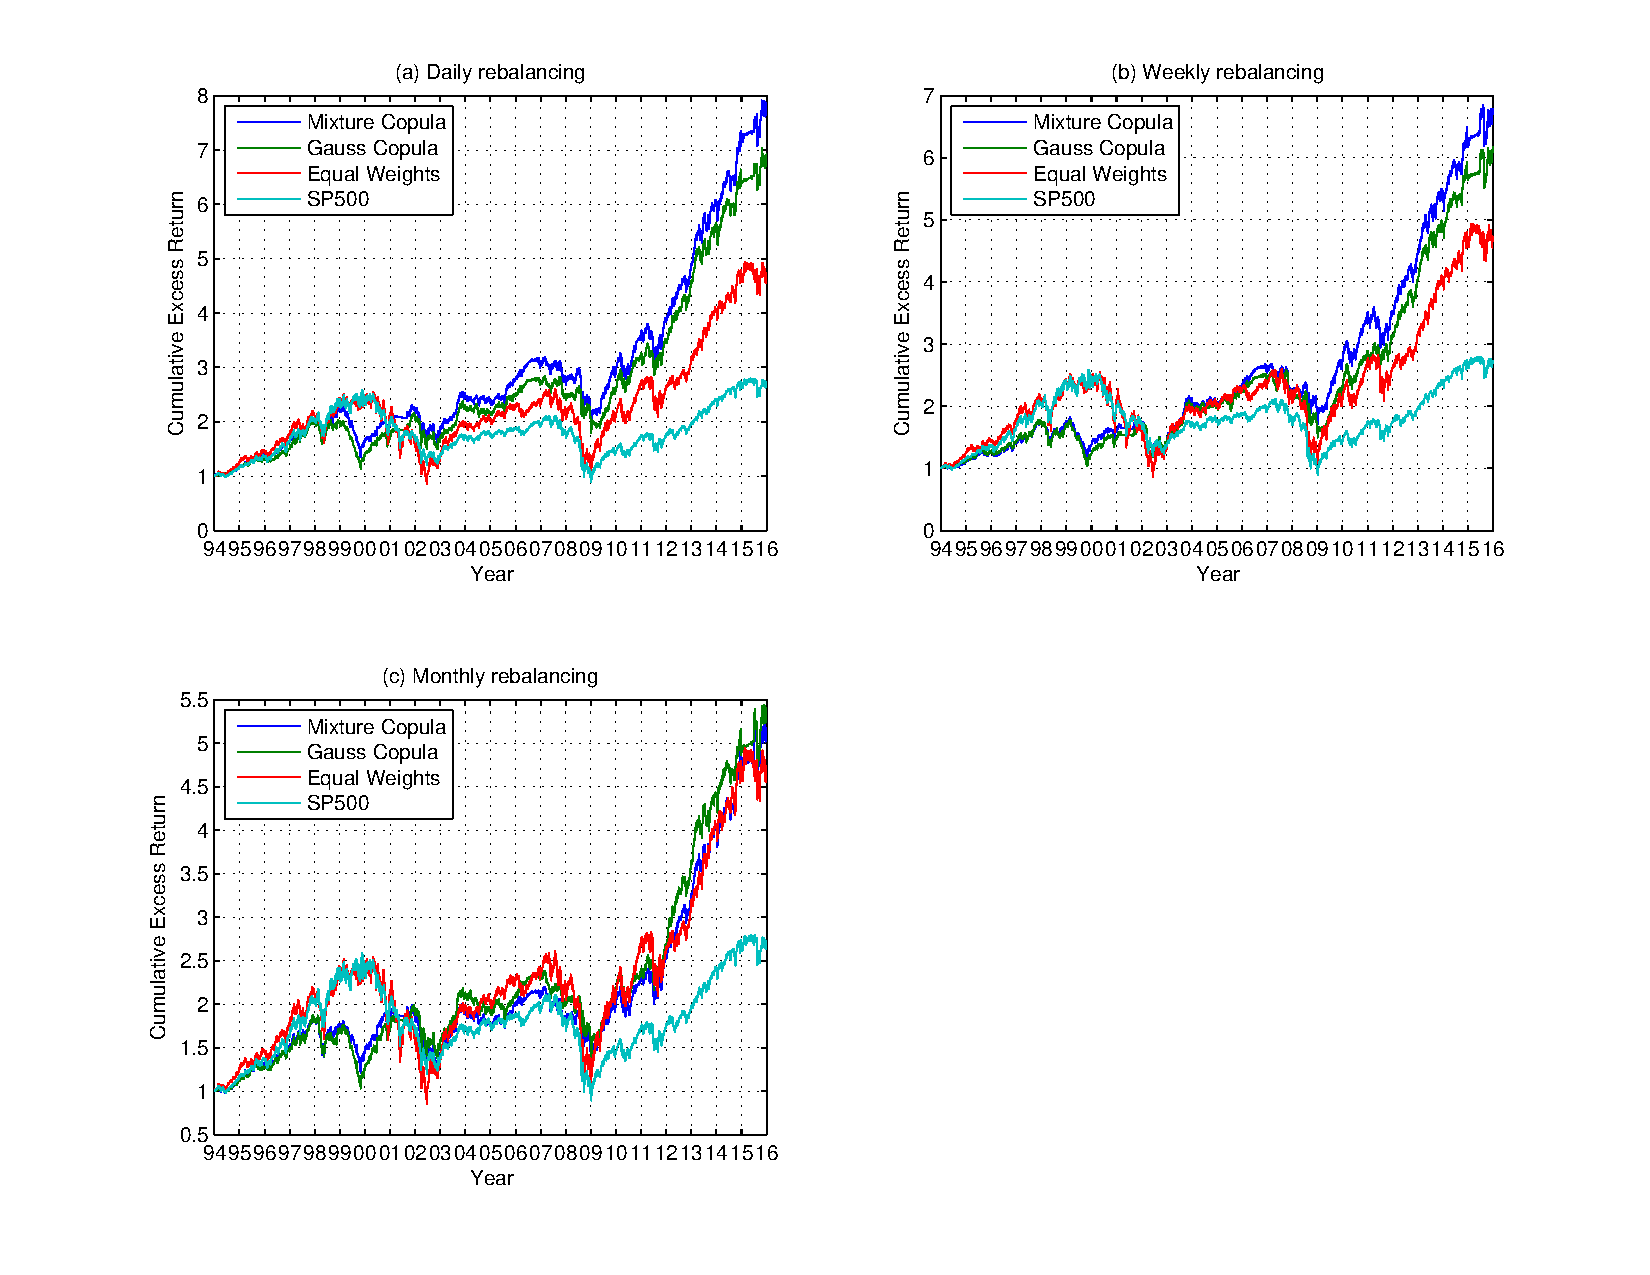
\includegraphics[scale=0.3]{fig1_rpwcop.pdf}
	\caption{\scriptsize Cumulative excess returns of the portfolio strategies without daily target mean return }
	\caption*{This figure shows how an investment of \$1 evolves from July 1994 to December 2015 for each of the portfolios.}
	\label{fig:fig01}
\end{figure}

The copula-based approaches are more profitable for daily and weekly rebalancing over time, especially after 2009. We can note the copula methods present a hump-shaped pattern in 1999, while the other benchmarks show a sharp decline in the subperiod that corresponds to the bear market that comprises the dotcom crisis and the September 11th terrorist attack (2000-2002). All portfolios show a hump-shaped pattern during the subprime mortgage financial crisis in 2007-2008. Overall, we can observe that after 2002 the patterns are similar, but the figure indicates that the copula methods, even though the objective function is the minimization of CVaR under a constraint on expected return, preserve more wealth in the long-term period, particularly the WCCVaR portfolio, for daily and weekly rebalancing \footnote{Transaction costs should not be neglected as we could notice after the breakeven analysis}.



\vspace{0.3cm}


\section{Conclusions}

In this paper we combine robust portfolio optimization and copula-based models in a Worst Case CVaR framework. To cope with the large number of financial instruments we employ a procedure similar to that used by \citet*{ggr06} to select a set of diversified assets that can be useful during crises and tranquil periods. Using data from the S\&P 500 shares from 1990 to 2015 we evaluate the performance of the WCCVaR (Worst Case Copula-CVaR) portfolio, considering different rebalancing strategies, and compare it against three benchmarks: a Gaussian Copula-CVaR (GCCVaR) portfolio, an equally weighted portfolio (1/N) and the S\&P 500 index. 

By selecting a diversified set of assets over a long-term period we found that copula-based approaches offer better hedges against losses than the 1/N portfolio. Moreover, the WCCVaR approach generates portfolios with better downside risk statistics for any rebalancing period and it is more profitable than the Gaussian Copula-CVaR for daily and weekly rebalancing.

Finally, we offer some suggestions for future research for improving our discoveries. First, we could improve the method of asset selection. We suspect that if we use a measure of nonlinear dependence between random variables of arbitrary dimension such as the randomized dependency coefficient (\citet*{lopez2013randomized}) or a procedure based on data mining tools as random forest \citet*{dlrz10} to select the stocks the portfolio performances would be even better. 
Additional suggestions include relaxing the assumption of no short selling and incorporate transaction cost as an additional constraint in the optimization problem as in \citet*{krokhmal2002}.
% Furthermore, a regular or a D-vine copula could add flexibility when modeling the dependence structure of the portfolio assets (even in higher dimensions), since they can describe a wider array of dependence patterns.

 %and investigate weekly and monthly return constraints.


\addcontentsline{toc}{section}{References}
\bibliographystyle{rfs}
\bibliography{mypapers}
\newpage

\end{document}
